%Document start and sets as a two column document
\documentclass[twocolumn]{article}

%%%%%%%%%%%%%%%%
%Used packages
%%%%%%%%%%%%%%%%

%For url usage in bibliogrpahy
\usepackage{url}

%Encodes input to utf8
\usepackage[utf8]{inputenc}

%Lorem ipsum language generator to check out layout of document
\usepackage{lipsum}

%Color source code
\usepackage{color}
\usepackage{listings}

%For plotting data
\usepackage{pgfplots}

%Used for keeping the table where I think it should be and not Latex
\usepackage{float}

%Title page
\title{\textbf{Spatial Distance Histogram Processing
	   of Large Scale Data} \\
	   University of South Florida\\
	   CIS 4930 - Summer 2016\\
	   Programming on Massively Parallel Systems}

\author{Kevin Wagner (wagnerk1@mail.usf.edu)\\
		Elijah Malaby (emalaby@mail.usf.edu)\\
		John Casey (jcasey2@mail.usf.edu)}
\date{July 1, 2016}

%Separates the columns by {<width>}
\setlength{\columnsep}{1cm}

%Sets the color of the source code
\renewcommand\lstlistingname{Quelltext} % Change language of section name

\lstset{ % General setup for the package
	language=Perl,
	basicstyle=\small\sffamily,
	numbers=left,
 	numberstyle=\tiny,
	frame=tb,
	tabsize=4,
	columns=fixed,
	showstringspaces=false,
	showtabs=false,
	keepspaces,
	commentstyle=\color{red},
	keywordstyle=\color{blue}
}


\begin{document}
	%Make the title section	
	\maketitle
	\newpage
	\tableofcontents
	
	%Turn page numbering on
	\pagenumbering{arabic}
	\newpage
  
%%%%%%%%%%%%%%%%%
%Abstract Section
%%%%%%%%%%%%%%%%%
\section{Abstract}
\par Graphic Processing Units (GPUs) today have a great deal of global memory a programmer can use for whatever reason deemed necessary. But what if the project and data at hand is too large even for the 2GB of the GTX 960, the 6GB of the GTX 980 TI, or even 12GB of the TITAN X card? Here the goal is to design an implementation of memory management systems or mechanisms to artificially limit the GPUs  global memory in an attempt to evaluate the effect of large data sets on the running time of a piece of kernel code.
\par Dividing and loading the data into global memory as blocks is unequivocally the easiest approach but, how the data is loading is going to be the challenging part of this experiment. Since data transfer from a host to a device's global memory is extremely costly, the efficiency of the data transfer is paramount.
\par{}To evaluate the kernel, the CUDA program will be run and the running time of the kernel will be plotted against data of different sizes.


%%%%%%%%%%%%%%%%%%%%%
%Introduction section
%%%%%%%%%%%%%%%%%%%%%	
\section{Introduction}
%I expect you to write a report in the format of a publishable paper. In the report, you should clearly state the objective of your project, your design of the data structure or algorithm, and relevant test cases by which the grader can evaluate your code.%
\par The objective of this project is to simulate the scenario where the data at hand is too large to all fit into global memory at once. This is a very large data set since some GPUs today come with up to 12GB of global memory on board. Loading the data is the trivial part of this project. The efficient loading of data is what this project is about. 
\par The expectation of the project is for the running times to be slower but, how much is the mystery. Loading to global memory is, as stated before, and extremely time comsuming process. An efficient algorithm to load data into the artificailly small global memory is again paramount and the results will solely depend on how this algorithm is implemented.
 
 
%%%%%%%%%%%%%%%%
%Strategies used
%%%%%%%%%%%%%%%%
\section{Strategies and Algorithms}
Starting with the code that was written for Project 2. Even with the best attempts in place the code was still 10x slower than what the Teaching Assistant(TA) had produced. Taking that into consideration, the project started with the TA's code in order to improve on that already optimized code. This code of course did not take into consideration if the data set was too large to fit into global memory of the GPU itself. 
\par Firstly, the na{\"i}ve solution was used. The data was loaded in global memory as blocks one after the other. 


%%%%%%%%%%%%%%%%%%%%%%
%Partial code examples
%%%%%%%%%%%%%%%%%%%%%%
\section{Code Examples}
\lipsum[1-3]
%example for code
\begin{lstlisting}
\end{lstlisting}
\lstinputlisting[language=C]{test_code.c}


%%%%%%%%
%Results
%%%%%%%%
\section{Results}
This section highlights the results obtained from our experiments and the control data we used to compare our data to.
\par \lipsum[1-2]

\subsection{Control}
For a baseline  to compare our experiments to we are using the data posted on CANVAS from the TA. Number of Atoms versus the Running time in seconds. See Tbl. 1 for the times and Fig. 1 for a graphical representation of the data.


\subsection{Experimental}
This section has the results we obtained in the project when we assume that the global memory is not big enough to hold all of the data that we have to to offer. We have to feed in the data a little at a time (say 200MB).



%%%%%%%%%%%%%%%%%%
%Test case section
%%%%%%%%%%%%%%%%%%
\subsection{Test Cases}
Thes

%%%%%%%%%%%%%%%%%%%
%Conclusion section
%%%%%%%%%%%%%%%%%%%
\section{Conclusion}
Go on about what we expected versus what we saw in testing. Does the loading of data the way we implemented it a success or failure? Go into some great detail why or why not.


%%%%%%%%%%%%%%%%%%%
%References section
%%%%%%%%%%%%%%%%%%%
\section{References}
\begin{enumerate}
\item NVIDA Corporation, CUDA Runtime API, 2015, http://docs.nvidia.com/cuda/cuda-runtime-api/index.html, [Online: accessed Summer 2016]
\item NVIDIA Corportion, CUDA Programming Guide, 2015, http://docs.nvidia.com/cuda/cuda-c-programming-guide/, [Online: accessed Summer 2016]
\end{enumerate}


%%%%%%%%%%%%%%%%
%Figures section
%%%%%%%%%%%%%%%%
\section{Figures}

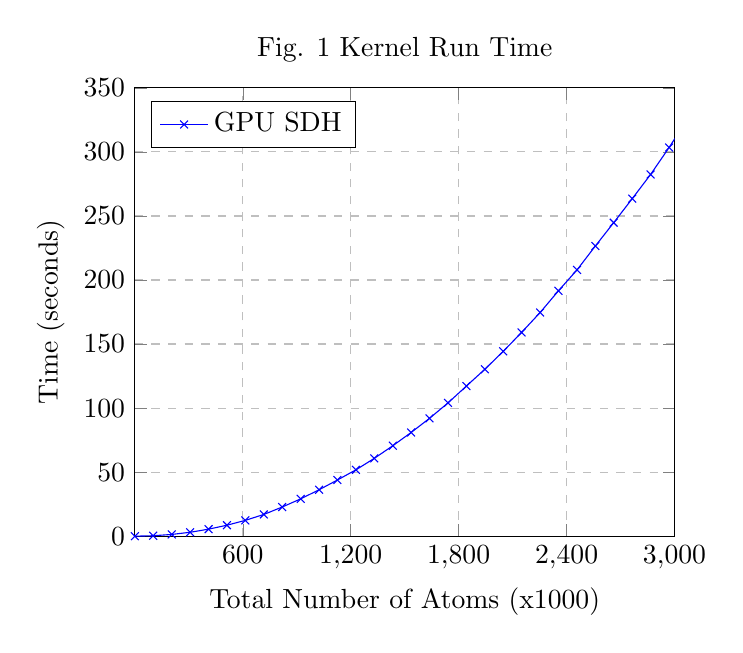
\begin{tikzpicture}
\begin{axis}[
    title={Fig. 1 Kernel Run Time},
    xlabel={Total Number of Atoms (x1000)},
    ylabel={Time (seconds)},
    xmin=0, xmax=3000,
    ymin=0, ymax=350,
    xtick={600, 1200, 1800, 2400, 3000},
    ytick={0,50, 100, 150, 200, 250, 300, 350},
    legend pos=north west,
    xmajorgrids=true,
    ymajorgrids=true,
    grid style=dashed,
]
\addplot[color=blue,mark=x,]
    coordinates {
    (0,0.001014944)
    (102,0.343783468)
	(205,1.360841751)
	(307,3.052339792)
	(410,5.48577261)
	(512,8.570511818)
	(614,12.34655285)
	(717,16.97405243)
	(819,22.75370407)
	(922,29.15684891)
	(1024,36.23521423)
	(1126,43.85413361)
	(1229,51.80871201)
	(1331,60.74640274)
	(1434,70.61425018)
	(1536,80.98942566)
	(1638,91.99478912)
	(1741,104.0754242)
	(1843,117.1748886)
	(1946,130.3655396)
	(2048,144.330658)
	(2150,159.09375)
	(2253,174.6193848)
	(2355,191.6004333)
	(2458,207.8615265)
	(2560,226.5615845)
	(2662,244.751297)
	(2765,263.5069275)
	(2867,282.3830566)
	(2970,303.4553528)
	(3072,325.8058472)
    };
    \legend{GPU SDH}
 
\end{axis}
\end{tikzpicture}

%%%%%%%%%%%%%%%
%Tables section
%%%%%%%%%%%%%%%
\section{Tables}
\begin{table}[H]
\caption{Run times for contol experiment}
\label{table:1}
\begin{tabular}{ |c|c|c|c| } 
\hline
Atoms & Time(s) & Atoms & Time(s) \\
\hline\hline 
512	& 0.00101494 & 1638912 & 91.99478912 \\
\hline
102912 & 0.34378347 & 1741312 & 104.07542420 \\
\hline
205312 & 1.36084175 & 1843712 & 117.17488860 \\
\hline
307712 & 3.05233979 & 1946112 & 130.36553960 \\
\hline
410112 & 5.48577261 & 2048512 & 144.33065800 \\
\hline
512512 & 8.57051182 & 2150912 & 159.09375000 \\
\hline
614912 & 12.34655285 & 2253312 & 174.61938480 \\
\hline
717312 & 16.97405243 & 2355712 & 191.60043330 \\
\hline
819712 & 22.75370407 & 2458112 & 207.86152650 \\
\hline
922112 & 29.15684891 & 2560512 & 226.56158450 \\
\hline
1024512 & 36.23521423 & 2662912 & 244.75129700 \\
\hline
1126912 & 43.85413361 & 2765312 & 263.50692750 \\
\hline
1229312 & 51.80871201 & 2867712 & 282.38305660 \\
\hline
1331712 & 60.74640274 & 2970112 & 303.45535280 \\
\hline
1434112 & 70.61425018 & 3072512 & 325.80584720 \\
\hline
1536512 & 80.98942566 & & \\
\hline
\end{tabular}
\end{table}



%End Document
\end{document}